%!TEX root = ../thesis.tex
\begin{savequote}[90mm]
	Scrum means ``Waterfall but we don't have time for analisys''\\
	Kanban means ``Scrum, but we don't have time for Sprint planning''\\
	Agile means ``We have no process but we do use Jira extensively''
	\qauthor{\href{https://twitter.com/mikeveerman}{@mikeveerman} on Twitter}
\end{savequote}

\chapter{Projet implementation}
\label{chapter_5}
	This chapter is the core of this document and describes the way that this project has been implemented according to the planning described in \Chapref{chapter_2}.\\
	It is structured in four main sections that go over the main time periods presented in the \Quote{Piano di Lavoro} document.\\
	Since the scope of the project was to create a demo environment to show the capabilities of Jira, Athonet has bought ten user licenses for Jira Software, ten for Service Desk and ten for Confluence.\\
	As described in Atlassian's documentation\cite{compare-atlassian-cloud-vs-server}, these tools have three installation options:
	\begin{itemize}
		\item \textbf{Cloud}: hosted on their infrastructure
		\item \textbf{Server}: download and install on a local network
		\item \textbf{Data Center}: download and install for a large infrastructure
	\end{itemize}
	Because of Athonet's policies about storing internal data in the cloud, the IT department opted for an on premise, Server, installation.
	This kind of installment requires a one time payment for the software while the subsequent fees will be for support.
\section{Learning phase}
	This phase corresponds to the first two weeks of the internship.
	As described in the \Quote{Piano di Lavoro}, the main task in this first period  was to understand what the tools are and what they can do.
	The first important thing to do was to acquire knowledge on Jira and Confluence by researching them on the Internet.
	The first one I have started researching was Jira, this brought me to the official documentation\cite{jira_docu}, which is very well organized.
	\begin{figure}[H]
		\centering
		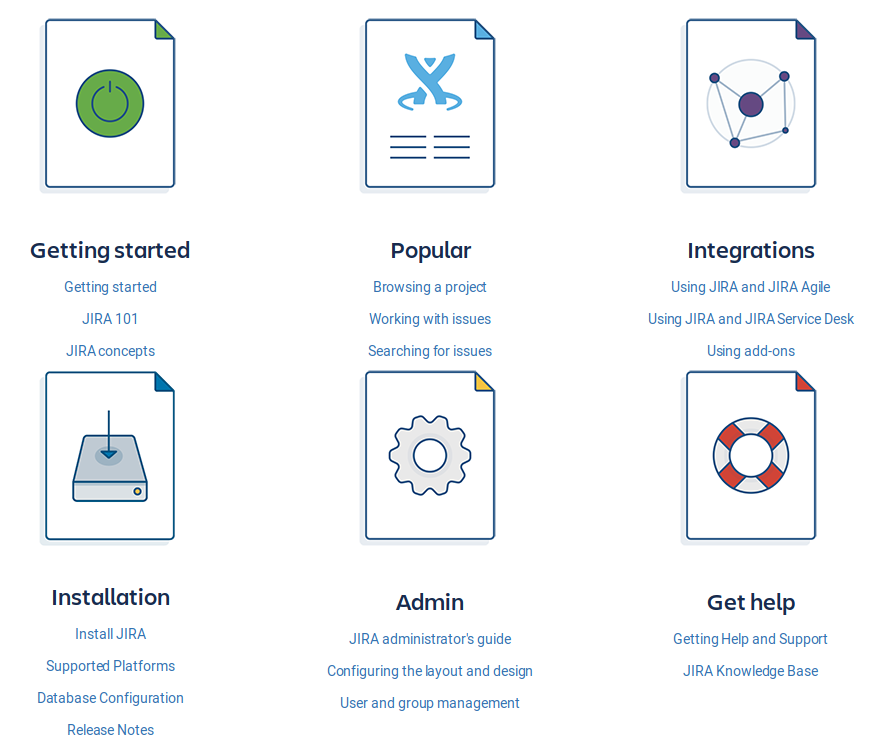
\includegraphics[width=1\textwidth]{resources/jira_documentation}\\
		\caption[Screenshot from Jira's Documentation page]{Screenshot of the sections from Jira's Documentation homepage from the Atlassian Support website}
	\end{figure}
	It is very easy to navigate because it's versioned for each release, major and minor, of the software, plus it contains links to related pages, including Confluence's documentation and Atlassian's blog.
	As said in \ref{sec:atlassian_community} both Jira and Confluence have a bug reporting and issue tracking section in their documentation.
	If a web page is related to an issue, this is showed at the end of the page with its status and a link to its dedicated section.\\
	The Confluence and Jira documentation are both written and hosted using a Confluence instance, showing how powerful can be this tool for handling a wiki for such a complex software that has a large userbase.\\
	Confluence's documentation is structured like Jira's, easy to access and consult, other than being public and free to read, despite the software are not.\\
	The second half of the first week was dedicated to configuring the environment.
	The IT department has chosen to create an instance of the Atlassian's software on a \gls{CentOS}\glsadd{CentOS} \gls{Virtual Machine}\glsadd{Virtual Machine} (VM) with 512GB of storage and 32GB of RAM, connected to a special testing network domain for internship students.
	The \gls{Remmina}\glsadd{Remmina} was used to remotely connect to the given VM.
	\begin{figure}[H]
		\centering
		
\includegraphics[width=.5\textwidth]{resources/centos_logo}\\
		\caption{Logo of the CentOS Linux distribution}
	\end{figure}
	
\section{Initial installation and configuration}	

	Since the exhaustiveness of the documentation, the installation phase was anticipated so that there could be a more hands on approach.
	As for the previous phase, the installation of Jira was done by following the dedicated article on the official documentation\cite{installing-jira-applications-on-linux}.	
	\begin{figure}[H]
		\centering
		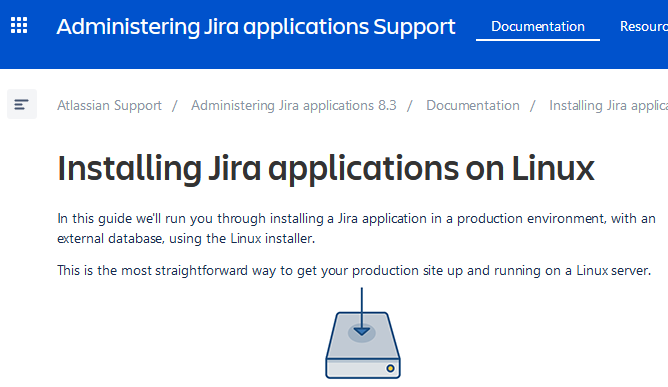
\includegraphics[width=.9\textwidth]{resources/jira_installation}\\
		\caption{Screenshot from the installation page of Jira in Atlassian's documentation}
	\end{figure}
	To store all the information regarding projects, users, etc., Jira needs a database.
	For the first installation, intended to be used in a testing manner, the embedded \gls{H2 database}\glsadd{H2 database} was enough.
	It's important to note that the documentation says the H2 database is not suitable for production environments\cite{accessing-jira-s-h2-embedded-database}.
	The first thing done after the installation was getting acquainted with the interface and understanding ho Jira's components interconnect with each other.\\
	In order to do this it was necessary creating some mock projects and filling them with issues.
	Here is where the concept of Board come out in Jira.\\
	Boards and workflows are very tied notions.
	Experimenting with workflows was one of the most important things to do, because these are fundamental in an Issue Tracking System's configuration and are strictly connected to Boards.
	\begin{figure}[H]
		\centering
		\makebox[\textwidth][c]{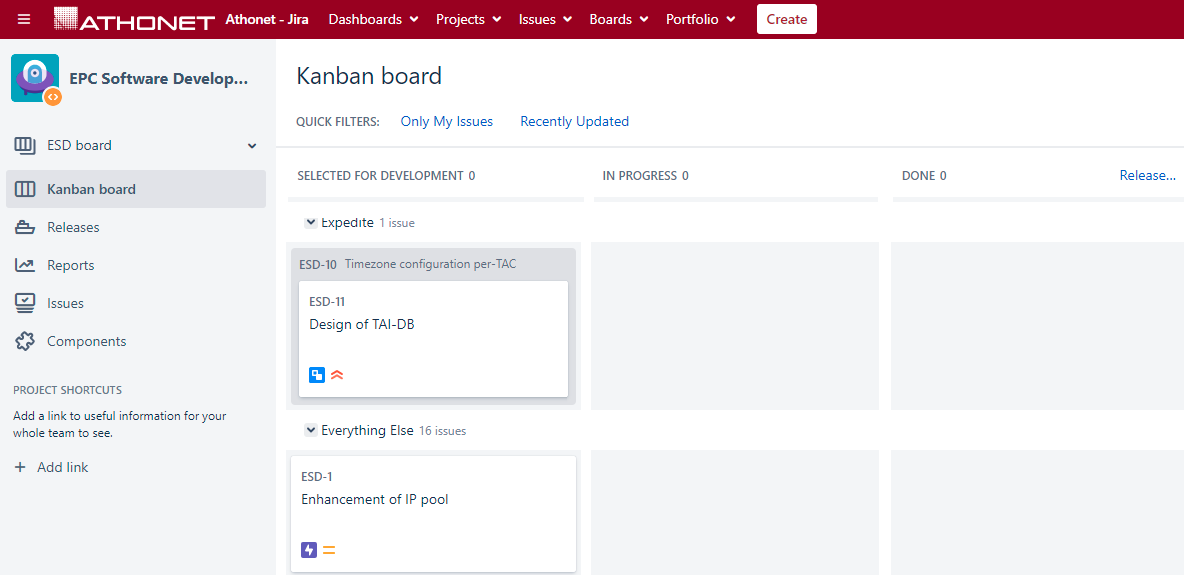
\includegraphics[width=1.2\textwidth]{resources/UntitledA}}%
		\caption{Kanban board from a Jira project}
	\end{figure}
	Installing Portfolio was the step that came after understanding the fundamentals of Jira and getting to know its basic features.
	This plugin, as told in \ref{subsec:portfolio} helps visualizing the issues on a roadmap, which was one of the most important requirements: \textit{O05}.\\
	As per the previous installation, Portfolio's was done by downloading and embedding the binary into Jira's instance.
	\begin{figure}[H]
		\centering
		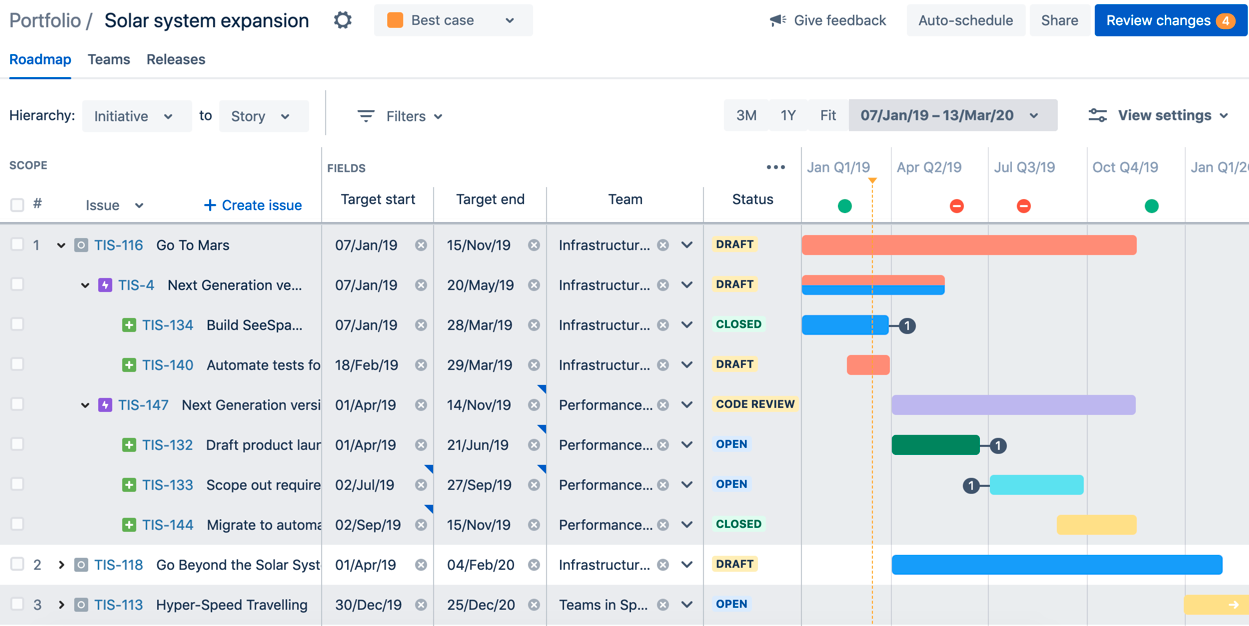
\includegraphics[width=\textwidth]{resources/portfolio}\\
		\caption[Screenshot of roadmap in a Jira Portfolio project]{Screenshot of roadmap in a Jira Portfolio project\cite{portfolio}}
	\end{figure}
	\begin{figure}[H]
		\centering
		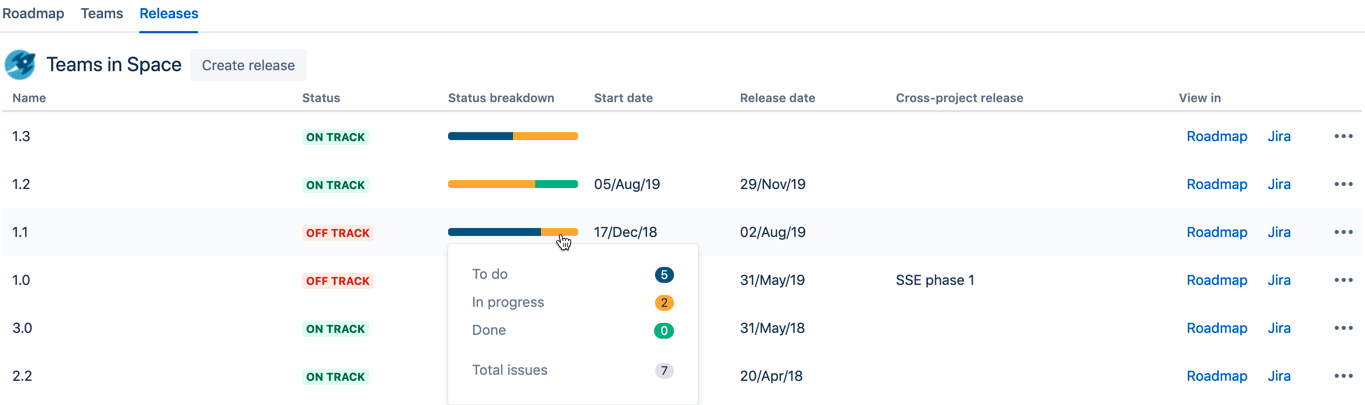
\includegraphics[width=\textwidth]{resources/IPS}\\
		\caption[Screenshot of releases in Jira Portfolio project]{Screenshot of releases in Jira Portfolio project\cite{portfolio}}
	\end{figure}
	The CTO of the company and PriMo's product owner were interested in the possibility of using a real time roadmap to keep track of the work done while not going as in deep as seeing the tasks assigned to each developer.\\
	After installing this plugin and creating plans for the previously created mock up projects, the next software installed was Jira Service Desk, to complete the configuration of the Jira instance.
	As described in \ref{subsec:service_desk} this piece of software is mostly used to communicate with the clients and having a portal from which a user can find information and request assistance with a product.
	In Jira Service Desk, the customer portal is the site where customers file and track requests.
	After installing this software, the first thin to do was creating a \Quote{Help Center} to see from the client's point of view how it can be able to open an issue and what types he may have access to.
	\begin{figure}[H]
		\centering
		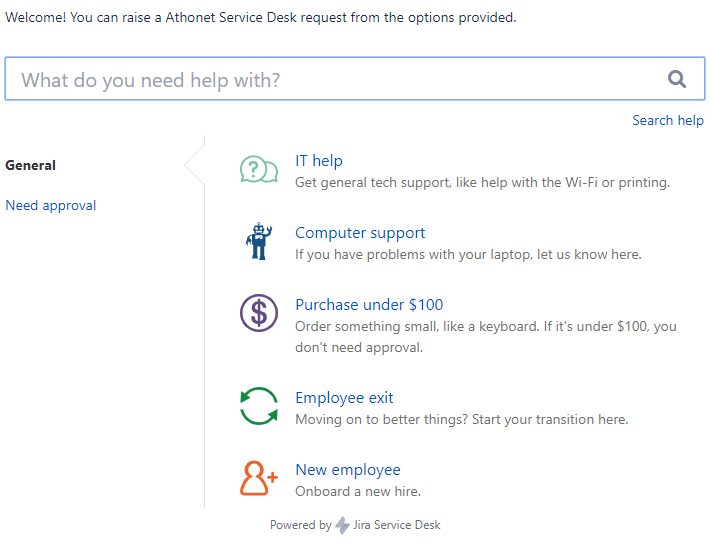
\includegraphics[width=\textwidth]{resources/Annotation2019-07-24170249}\\
		\caption{A Jira Service Desk portal}
	\end{figure}
	The installation of Confluence came after understanding all the basics of Jira and becoming familiar with it.
	For the newly installed software the H2 database was enough as for the previous one.
	Both software run on the same system, and their services are offered on port 8080 and 8090 respectively for Jira and Confluence via HTTP protocol.\\
	During the installation of Confluence, the install wizard program allowed me to insert all data of the Jira instance in order to connect them.
	A knowledge base for the Service Desk project and a documentation space for the Software project have been generated in order to test the connection.\\
	To allow a better integration between these tools, Atlassian allows to have a single database table containing the users information stored on either one of Jira or Confluence's instances.\\
	This was shown during the installation of Confluence as an option to link it with Jira's instance was presented by asking for the administrative credentials for connecting to the database and using Jira's users.
	Jira and Confluence both use the open source Apache Tomcat web server.
	This particular web server has issues regarding the login when both software run on the same IP address: each program stores \gls{cookies}\glsadd{Cookie} to allow users to log in without inserting each time username and password.
	On each log in though, users were automatically logged out of the system almost immediately.
	After a research on the Internet I found a post\cite{user-is-constantly-logged-out-of-jira} in Atlassian's blog regarding this problem: the answer was that when run on the same IP address, cookies from Jira and Confluence go in conflict.
	This post was associated with a more detailed issue\cite{JRASERVER-36960} in Jira's own portal.\\
	The solution to this problem was to change the \gls{context path}\glsadd{Context Path} of both applications\cite{how-to-change-the-jira-application-context-path} in the \Quote{server.xml} file that contains the configuration of the web server.
	An example of changing the context path is:
	\begin{center}
		\texttt{http://yourdomain.com:8080}
	\end{center}
	\vspace{-10pt}
	becomes:
	\vspace{-10pt}
	\begin{center}
		\texttt{http://yourdomain.com:8080\textbf{/jira}}
	\end{center}
	For Confluence, where the default port is 8090, the context path would become:
	\begin{center}
		\texttt{http://yourdomain.com:8090\textbf{/confluence}}
	\end{center}
	Contrary to what was said in the beginning, the tutor had communicated me that the IT department opted to maintain for using GitLab\cite{gitlab} instead of installing BitBucket\cite{bitbucket}, another Atlassian software.	
	This because GitLab was already in use by the developers, so they would not need to learn a new software that could affect their work routine.
	\begin{figure}[H]
		\centering
		\includegraphics[width=.5\textwidth]{resources/glan}\\
		\caption{GitLab Logo}
	\end{figure}
	Connecting these tools together means that a developer can interact with Jira's issues from a GitLab project by typing it's ID in the messages that he uses for commits, comments, merge requests and so on.
	GitLab's documentation has a dedicated page with instructions, examples and a guide that allow configuring both tools\cite{integrations}.\\
	This functionality allows GitLab to interact with Jira's default workflows, which sometimes are too simple for some software projects.\\
	Since the license for GitLab's hosted version is not \Quote{Premium} (or \Quote{Silver} for the online one) there is no interaction the other way around, from Jira to the repository\cite{jira_development_panel}.
	Since these tools are not strictly related, there is no direct project mapping from GitLab to Jira, a commit message in the repository may reference multiple Jira issues from different projects, so it's the programmer's discretion to comment wisely.
	Later in the text it's described the installation of a plugin that allows these tools to connect with more functionalities.\\
	A demo that touched all the previously viewed arguments was set in place for showing the progress made to the tutor.	
	Because his availability at the moment was very little, from the time the meeting was set to the actual moment of it happened, the interface of the system was customized by adding the colors of the company and its logo.
	\begin{figure}[H]
		\centering
		
\includegraphics[width=\textwidth]{resources/jira_custom}\\
		\caption{Custom menu interface for Jira}
	\end{figure}
	\vspace{-.5cm}
	\begin{figure}[H]
		\centering
		
\includegraphics[width=.85\textwidth]{resources/confluence_custom}\\
		\caption{Custom menu interface for Confluence}
	\end{figure}
	During the meeting, the tutor liked the progress that was made and asked for more elaborate mock projects for presenting the tools' combined functionalities to other company figures.\\
	The projects registered until that moment in Jira and their related spaces in Confluence were deleted and, as hinted in \ref{sec:time_planning}, a snapshot of the VM hosting the software was taken.\\
	Until this point the completely fulfilled objectives were: \textit{O01}, \textit{O02}, \textit{O05}, \textit{D03}.\\
	Although the connection between Jira and GitLab was established, to fulfill O04 it was required that GitLab supported custom workflows for Jira Software projects.
	
\section{First realistic mock projects and feedback}

	The previous paragraph marked the first three weeks of the internship.
	Starting the fourth week the task was to implement more realistic projects in Jira, connecting them to Confluence providing them with documentation and creating a link with GitLab.
	The objective was to expand the demo so that it could be shown to other members of Athonet to understand, both me and them, how these software can be used in their departments.\\
	The new Software projects created in Jira were called \Quote{EPC} and \Quote{Dashboard}, linked to their documentation spaces in Confluence, respectively \Quote{EPC Documentation} and \Quote{Dashboard Documentation}.
	To show the functionalities of Jira Service Desk as a knowledge base portal (sharing internal documents between employees), the \Quote{Athonet Internal Wiki} project was created.\\
	For the first project a more articulate workflow has been implemented to resemble the realistic evolution of an issue inside the company.
	\begin{figure}[H]
		\centering
		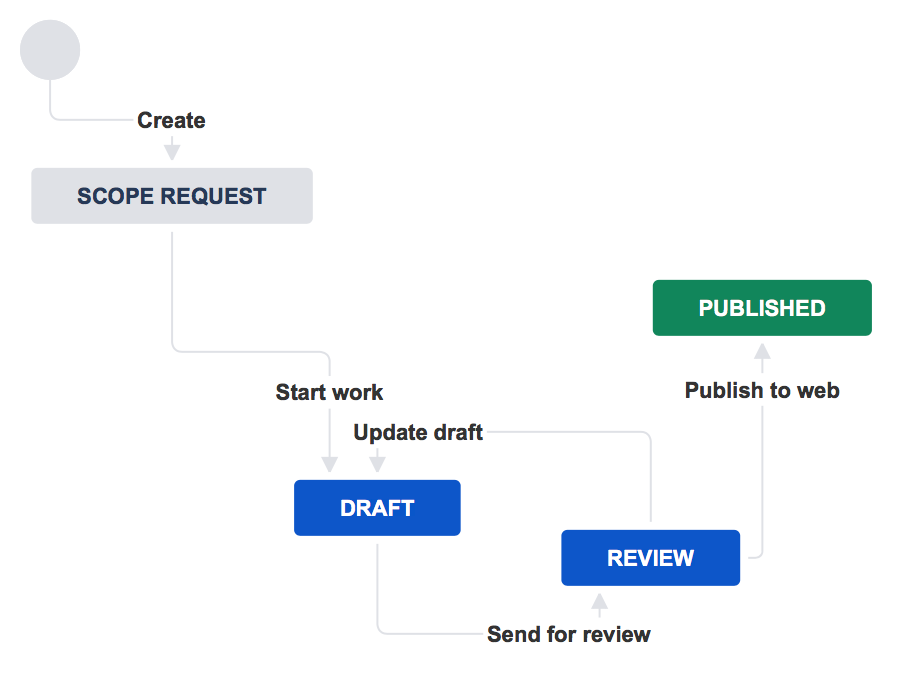
\includegraphics[width=.7\textwidth]{resources/Web+update+workflow}\\
		\caption{Custom example workflow that can be implemented in a Jira project}
	\end{figure}
	While working on the mock projects and creating issues, it was useful to note down all the most important customization that an administrative user can use to set up the software, not only for Athonet's specific purposes but in general.\\		
	To make the project more realistic three new user groups were created, besides the default ones, to which there were assigned three users each:
	\begin{itemize}
		\item Management
		\item Verification
		\item Developers
	\end{itemize}
	Every group had custom permissions allowing to demonstrate how basic security rules work in these tools (requirement \textit{D06}).\\
	A first draft of how the menu for creating a new issue can be customized was done as well, although not final (requirement \textit{D05}). 
	\begin{figure}[H]
		\centering
		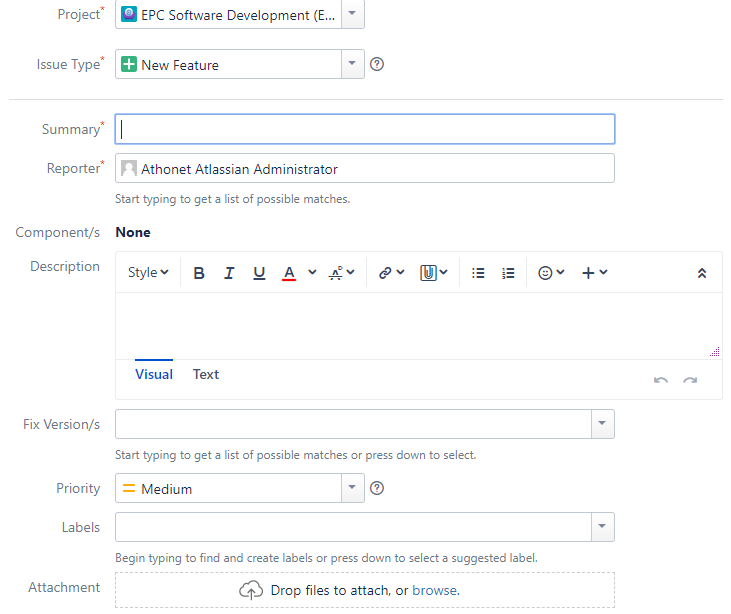
\includegraphics[width=.9\textwidth]{resources/Annotation2019-07-24170502A}\\
		\caption{Draft for custom issue creation and editing menu in Jira}
	\end{figure}
	After talking to the tutor about the made, he was able to set a meeting with himself, the verification and developer managers.
	Slides were prepared in order to explain the nomenclature in Jira, described in this document in \ref{sec:concepts}, and the features that have been paired to the demo projects.\\
	The core of this meeting was a discussion between the managers focused on understanding how their ongoing projects in Redmine could be implemented in such a way that the employees would not be forced into using a strict Agile methodology, but to accommodate and let them understand how these tools work without creating chaos.\\
	There was a discussion on how applying a strict Agile methodology could impact their time division.
	Agile provides sprints that by definition last two weeks, and these produce deliverables that bring added value to the project.
	Athonet's line of work though is focused on adding value to the product upon new releases that are scheduled differently by their purpose:
	\begin{itemize}
		\item Bug fix
		\item Minor release (for patching issues with the code or to improve performance)
		\item Major release (for new features)
	\end{itemize}
	Sprints would disrupt the routines of their developer team, the verification team and of management.
	In this case it would not be the tool that adapt to the company but vice versa the company would need to change in order to use the tool and would result counterproductive.\\
	The developer manager stated that he wanted a way to measure productivity, so I showed him the \Quote{Reports} section that is present for all kind of Jira projects.
	Here there are the burndown report charts that have been explained earlier in the text, in \ref{sec:metrics}.
	\begin{figure}[H]
		\centering
		\makebox[\textwidth][c]{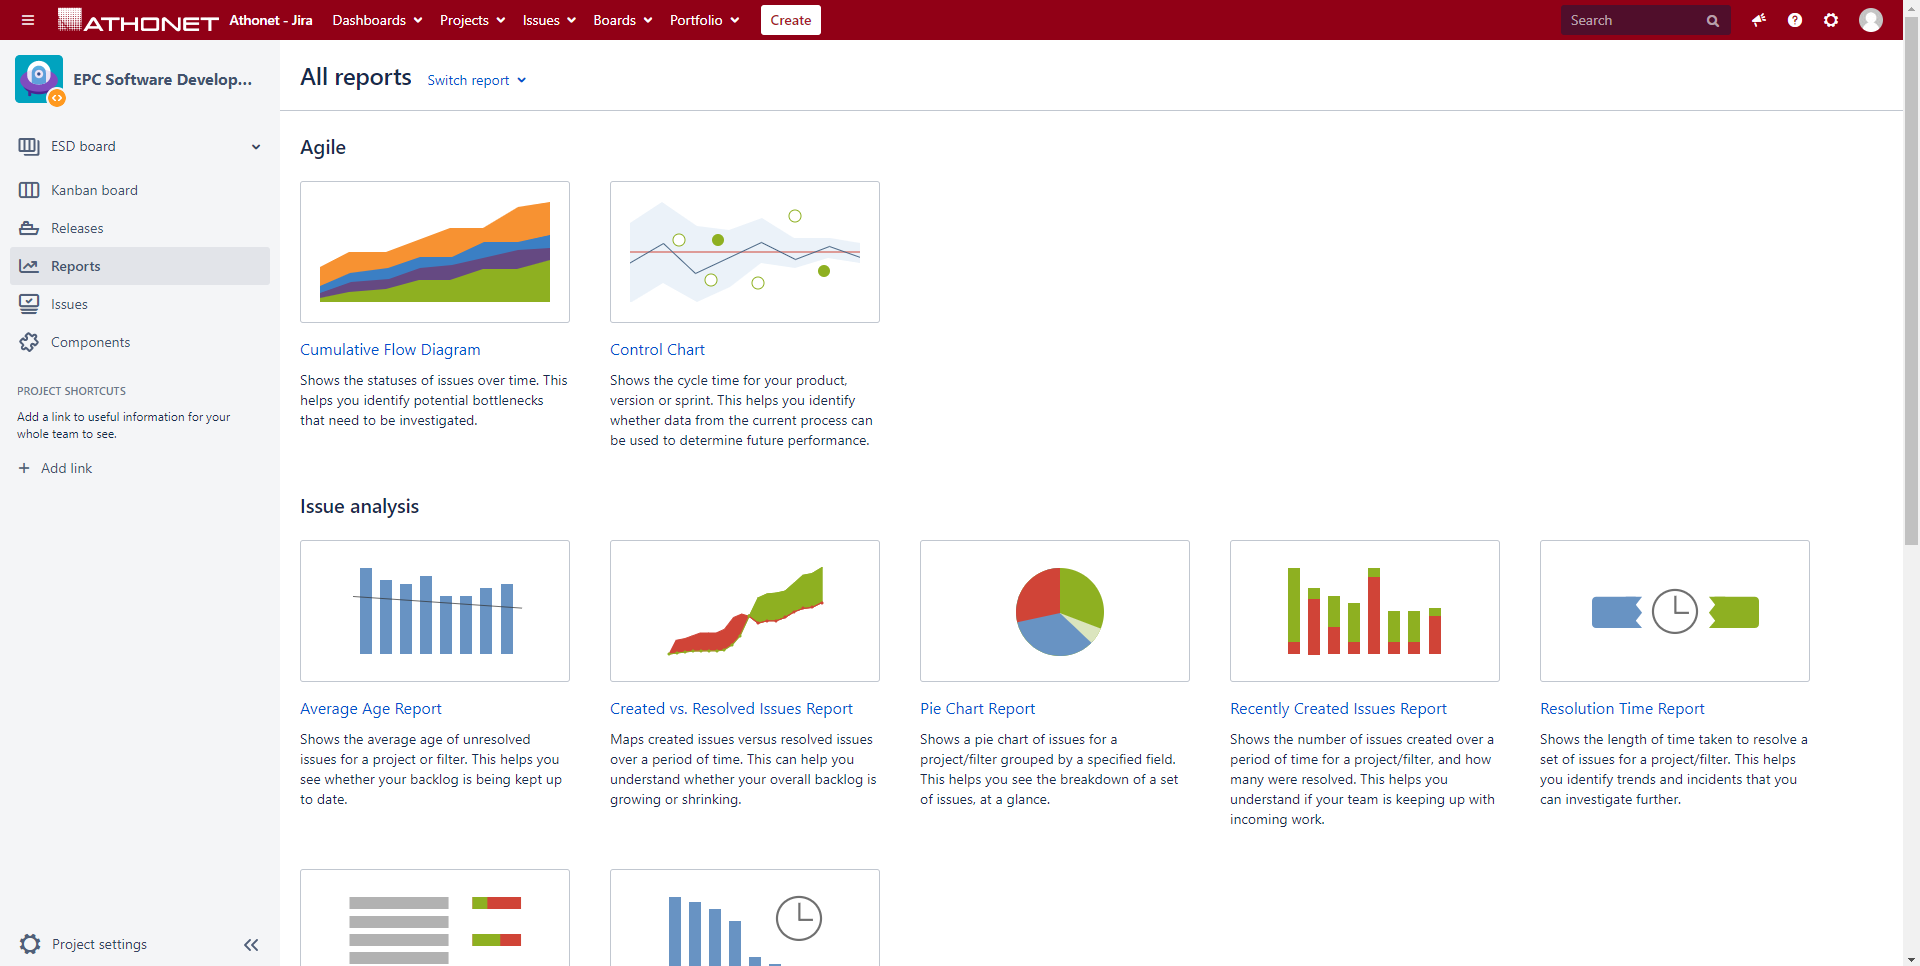
\includegraphics[width=1.2\textwidth]{resources/Annotation2019-07-24180041}}%
		\caption{Kanban board from a Jira project}
	\end{figure}
	Both managers were more pleased to see that Kanban boards resembled better their way of working, even if they want to maintain some of Scrum's peculiarities.
	The developer manager also said that it would be better for the company's way of working since developers could plan their tasks based on what has to be completed for the next release, so for a longer period of time.\\	
	This implied there would be a more particular workflow that had to be implemented and the managers were pleased to see that it could be easily done, as for customizing the issue creation and modification menu.\\
	They were also glad about the internal wiki project because it suggested there could be one single tool for both internal documentation regarding clients and general notes for employees.
	The following image is an example of how an article is visualized in this wiki.
	\begin{figure}[H]
		\centering
		\makebox[\textwidth][c]{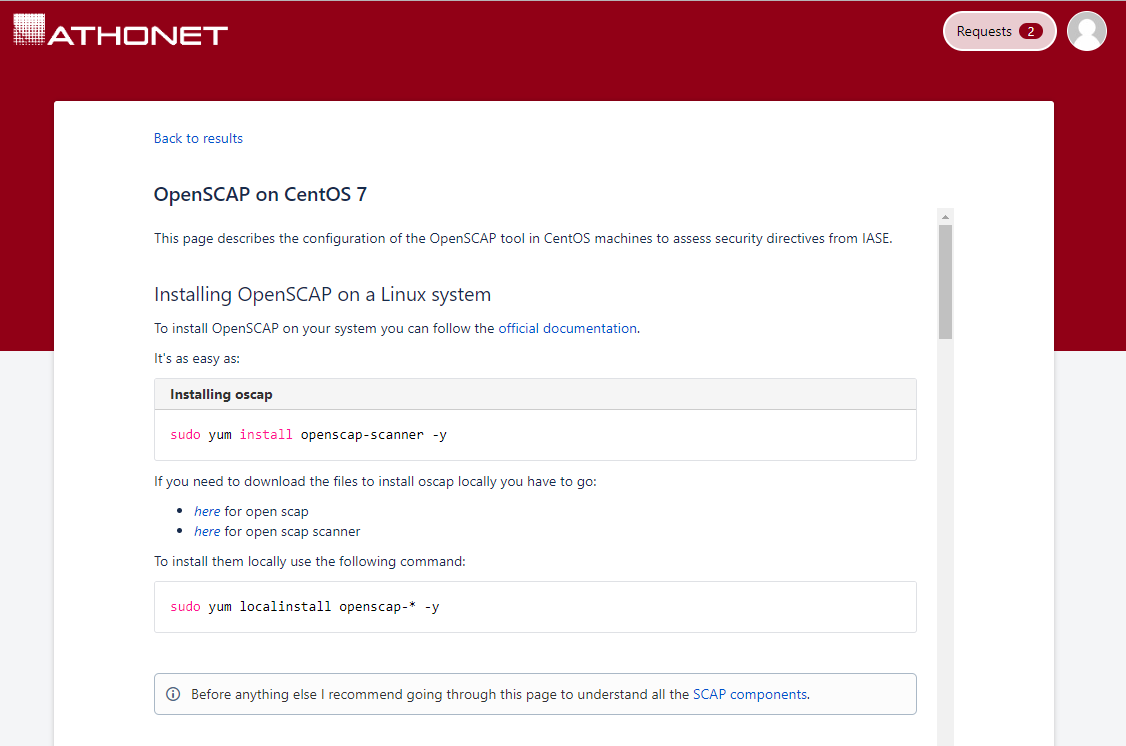
\includegraphics[width=1.1\textwidth]{resources/Annotation2019-07-2470331}}%
		\caption{Screenshot of article in Jira Service Desk}
	\end{figure}
	Articles like this correspond to pages written in a Confluence knowledge base space connected to the Service Desk project.
	\begin{figure}[H]
		\centering
		\makebox[\textwidth][c]{\includegraphics[width=1.1\textwidth]{resources/Annotation2019-07-24180113}}%
		\caption{Screenshot of a page in Confluence that is being edited}
	\end{figure}
	The company members needed time for internal discussions that had to be done in order for the managers to understand how to adapt the workflow they had in Redmine for Jira and how to include Confluence in the mix.
	In this period the documentation was elaborated, anticipating it from the original plan in the \Quote{Piano di Lavoro}.\\
	The first one to be produced was the \Quote{Installation an Configuration Guide}, written for the IT administrators and the people that would maintain, configure and eventually reinstalled if needed, the software.
	After this was drafted and approved from the tutor, I worked on the \Quote{Final User Guide}, written in the wiki Confluence that was previously demoed.
	Both regarding requirement \textit{O03}.
	Later on, a new meeting was scheduled with the product owner, who wanted to understand better Portfolio and how the concept of \Quote{product} matches the \Quote{project} denomination in Jira.\\
	Project and product sound similar and the two concepts are often confused with each other.
	A project is a temporary endeavour, with a clear definition of what needs to be delivered and by when, it has a beginning and end date.
	A product is designed to continually create value for customers by solving their problems\cite{product}.\\
	For the product owner, one of the most important things was to see how releases are mapped inside the software, since Redmine did not offer such an intuitive interface and did not allow to see them on a timeline and applying custom filters.
	He approved the progress made after seeing it and also said that he wanted the credentials to start using the software and see how to map the ongoing projects in Redmine to new ones in Jira or how to eventually migrate them, as per requirement \textit{F02}.\\
	After using it for a couple of days and talking with the other managers, he told me how they want to implement the evolution of an issue.
	Since they were not sure letting users access Service Desk directly, an employee would create an issue that would represent the customer request through service desk.
	The customer request could be a new feature, a bug report, require support, etc.
	This would then be picked up by a team that would bring it inside a Business type of project by creating a linked issue.
	This project would have a particular workflow and contains the more high lever tasks like documentation, meeting notes, feature statuses, etc.
	These shared notes and documents would be stored in Confluence, where there would be links to them.
	After they have been approved for production another team would create a linked issue inside the software project.
	This would most likely be divided in many sub-issues by the team leader and these would be visible by the developers.
	Each developer could then pick an issue to work on and handle it as he wants by, for example, dividing it in smaller sub-issues.\\
	The next week another meeting was scheduled with more company figures: a senior developer, the business strategy manage, the managers from the previous meetings, the CTO and the tutor.\\
	As in the other meetings I have presented the software, the major use cases and progress done, referencing the objectives achieved and showing them the working system by creating issues in projects that would resemble the way of working described by them.\\
	Even with the requirements changes that occurred, I was on schedule with the planning, a more detailed view can be seen in the Gantt diagram in \ref{gantt_2}.
	\newpage
	\begin{landscape}
		\vspace*{\fill}
		\begin{figure}[H]
			\centering
			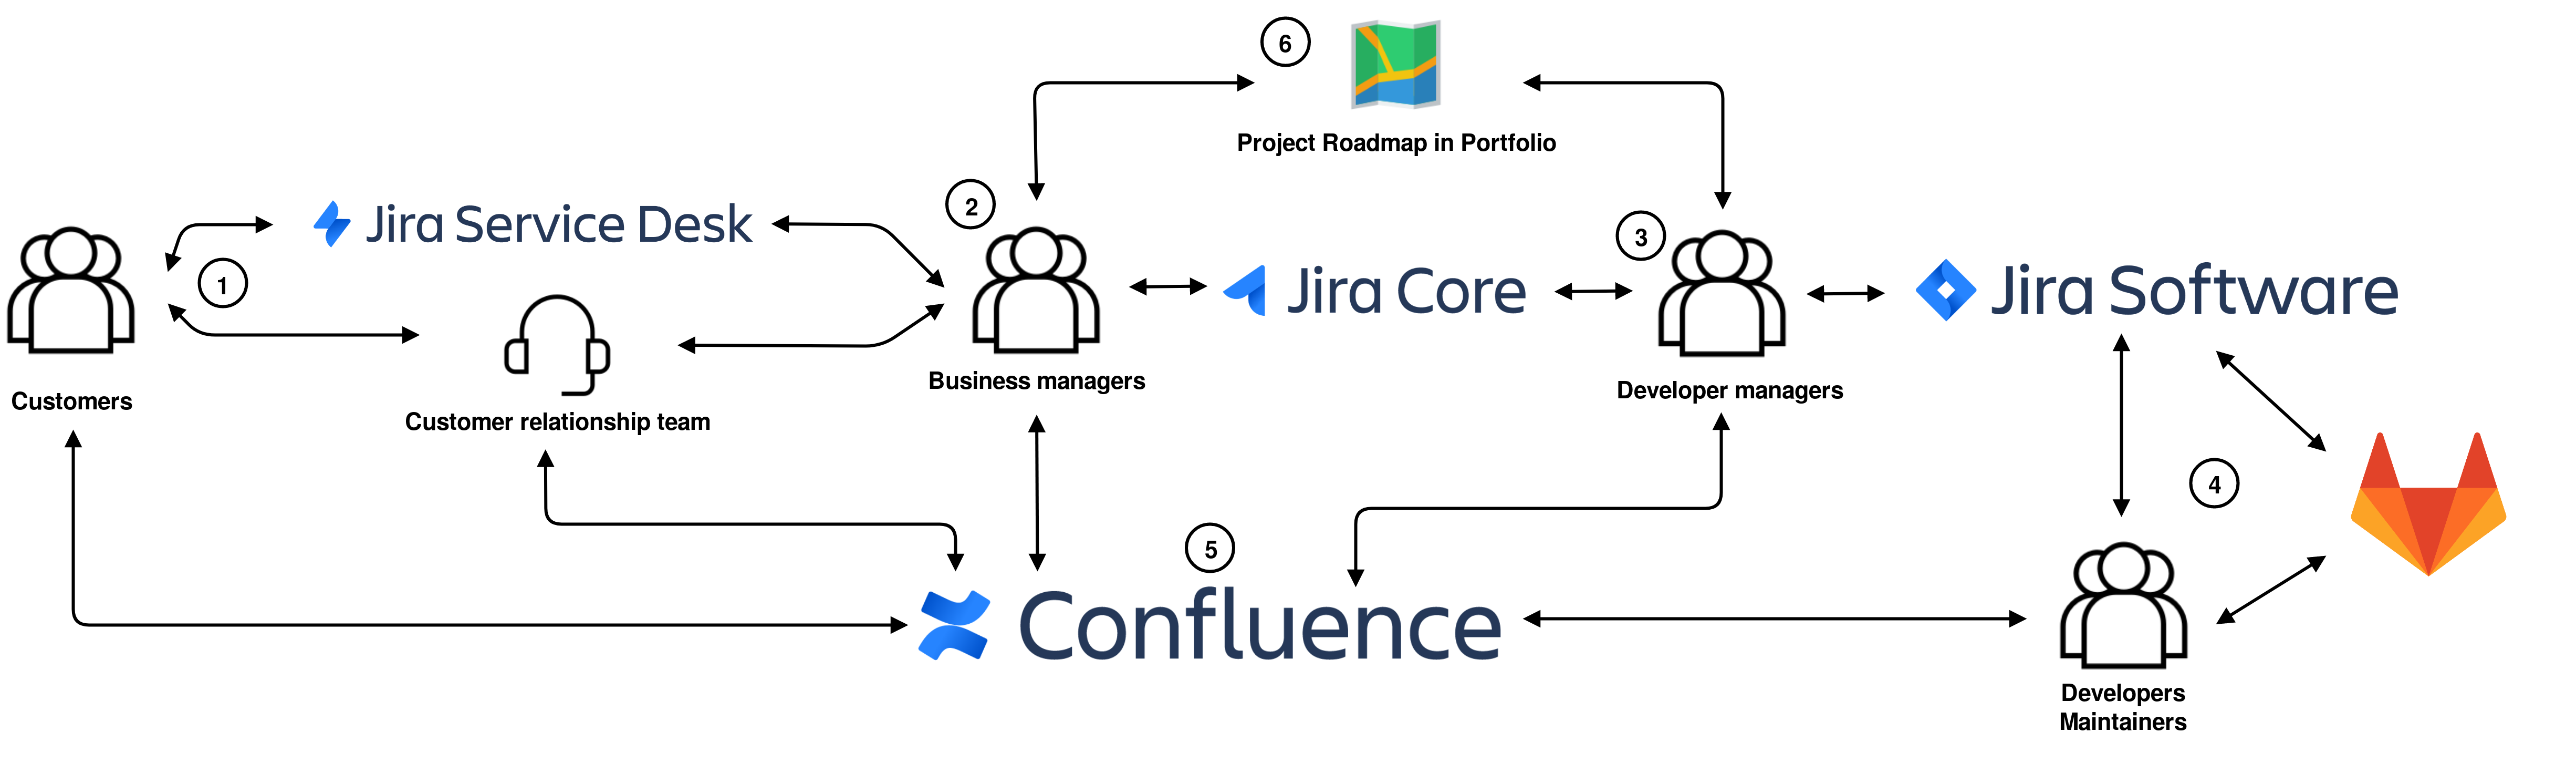
\includegraphics[width=22cm]{resources/UntitledDiagrammmmm}\\
			\caption{Evolution and transitioning of an issue}
		\end{figure}
		The main steps that an issue passes are:
		\begin{enumerate}
			\item The customer reports a bug or feature request to the Customer Relationship team or through a Jira Service Desk project
			\item The request is then picked up by the Business managers that discuss it and link it to a Jira Core issue in a dedicated project
			\item The features that are ready to be developed are sent in the Jira Software project by the development team managers
			\item The developers choose what to work on and commit to GitLab, which is connected with Jira Software, using special keywords
			\item Confluence is fully connected with every other Atlassian tool and allows users to store notes and documents
			\item Jira's Portfolio plugin is always up to date with the status of the issues and can be consulted by the managers (or developers)
		\end{enumerate}
		\hfill
		\vspace*{\fill}
	\end{landscape}
	\newpage

\section{Transitioning into Production and final feedback}

	To better connect GitLab with Jira the plugin \Quote{GitLab Listener}\cite{gitlab-listener} was installed.
	This allows for wider connectivity between the two products supporting custom workflows and more transitions with commit messages like:
	\begin{center}
		\texttt{New version \#refs ALLGEN-12 GTTSLT-2 \#time 1h 15m \#action ToDone}
	\end{center}
	This kind of command references two issues in two different Jira projects, telling the time spent and transitioning both to the \Quote{Done} column.
	Installing this plugin allowed to completely fulfill requirement \textit{O04}.
	\begin{figure}[H]
		\centering
		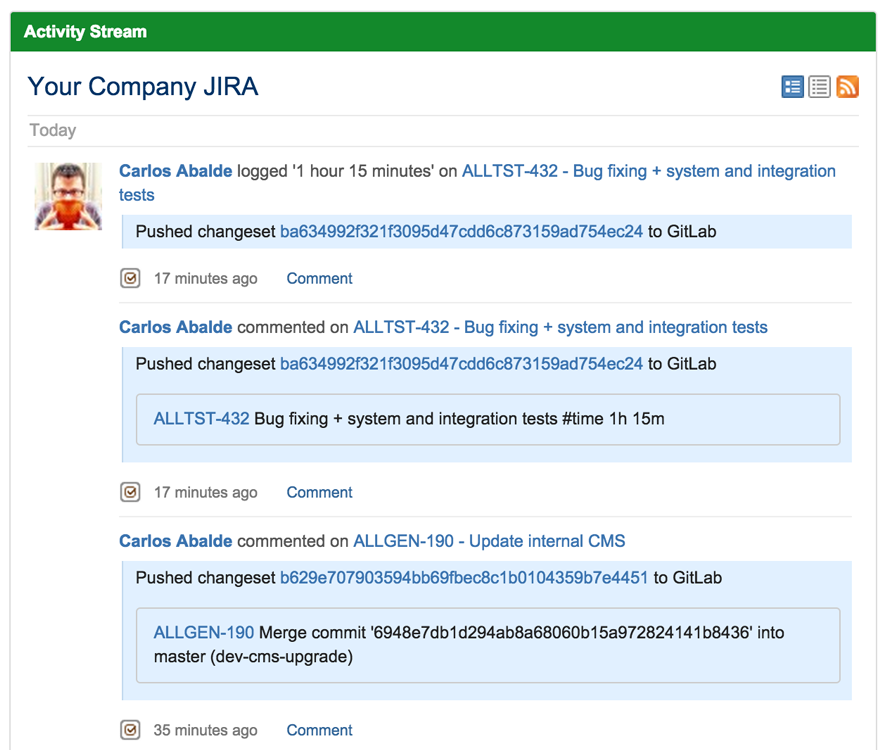
\includegraphics[width=.7\textwidth]{resources/aiaiai}\\
		\caption[Screenshot of how GitLab's messages are seen in Jira's interface]{Screenshot of how GitLab's messages are seen in Jira's interface\cite{gitlab-listener}}
	\end{figure}
	Although in the first planning this was a longer period of time, this last phase was shortened.
	This was due because of the many internal discussions that took place for the software to be approved and for the various managers of the departments to understand how to introduce it to their subordinates.\\
	After the last meeting, described in the previous paragraph, new users were created for the managers that participated and the credentials were given so that they could see the interface and interact with the mock projects that remained there.\\
	The tutor had credentials as well and he was very enthusiast of how the demo performed and the potentials of the software, although this had to be well understood by the other managers and members of the company as well.\\
	Although the last snapshot of the VM that was made contained a working infrastructure ready to be moved in a production environment, the IT department opted to wait until they understood how to properly secure the server that was going to host it.
	The most important part would be creating a secure \gls{VPN tunnel}\glsadd{VPN} that would allow employees that are working from other locations outside the company to connect as if they would be inside the building.
	This method must ensure thought that there would be no possibility for any other to get, or even hack, inside the company's network and access their products' source code.
	Besides this, the other managers where glad to hear that the tools have been approved and where happy about the demonstration.\\
	Because of this restrictions from the IT department, some of the requirements could not be fulfilled: \textit{D01}, \textit{D04}, \textit{F01}, \textit{F02}.
	These requirements could not be fulfilled because of the restrictions imposed by the IT department for interns.\\
	It would have required me to access their production server and having access to the data that is contained in the Redmine instance, which is available only for the employees.
	Or in case of \textit{D01} I could not fulfill the requirement because I would have needed access to the administrative passwords of Office 365.\\
	
\section{How are these tools being used}
	Even if Athonet does go for a pure Agile development model, the tools it has chosen to use still help to improve the organization of their work.
	In fact, the tools fits their current needs, which reflect an hybrid model between Scrum and Kanban: \Quote{Scrumban}.
	As in Kanban it helps visualizing workflow, limiting work in process (WIP), and measuring productivity are prioritized.	
	Scrumban removes the practice of limiting WIP by time (i.e. velocity and Sprint boundary) and replaces it by limiting WIP for each stage.
	It's based on having a continuous flow of work, which is what Athonet has for their products.\\
	In Jira, this methodology is called \Quote{Kanplan}\cite{kanplan}, and it is well documented on the \Quote{Agile Coach} section on their website.